\chapter{Results and Analysis}
\label{chap:results}
\section{Single Metrics}
\subsection{Scatterplots}
\label{sec:single_metrics}
We first visualize the results by plotting scatters of the metrics individually against the measured utility obtained by the different classifiers in Figures \ref{fig:metrics_scatter1}, and \ref{fig:metrics_scatter2}. This will help us get an idea of what to look at that and how to later quantify our findings. Every row represents a metric and columns are split between classifiers. Every scatterplot contains a line of best fit per dataset and the different datasets are separated by color. The gradient of these lines represent how changes in utility are reflected in the metrics. Broadly, we address the following: 
\begin{itemize}
    \item Per dataset, every metric tends to be separated into two disjoint point clusters, corresponding to the different algorithms
    \item For a metric, consistency, or lack thereof, across the datasets
    \item For a metric, consistency, or lack thereof, across the classifiers
    \item Some metrics have no linear correlation
\end{itemize}

These four points provide evidence for the limitations of individual metrics in predicting utility for $k$-anonymous datasets. Consistent trends are necessary for a metric to be useful because they represent how changes in utility are reflected in the metric. We need to be able to compare two different values for a metric and know what that difference in value implies for an arbitrary combination of dataset, algorithm, and classification task. The results show that we cannot do this with our metrics as we obtain inconsistent trends.

\begin{figure}
    \centerfloat
    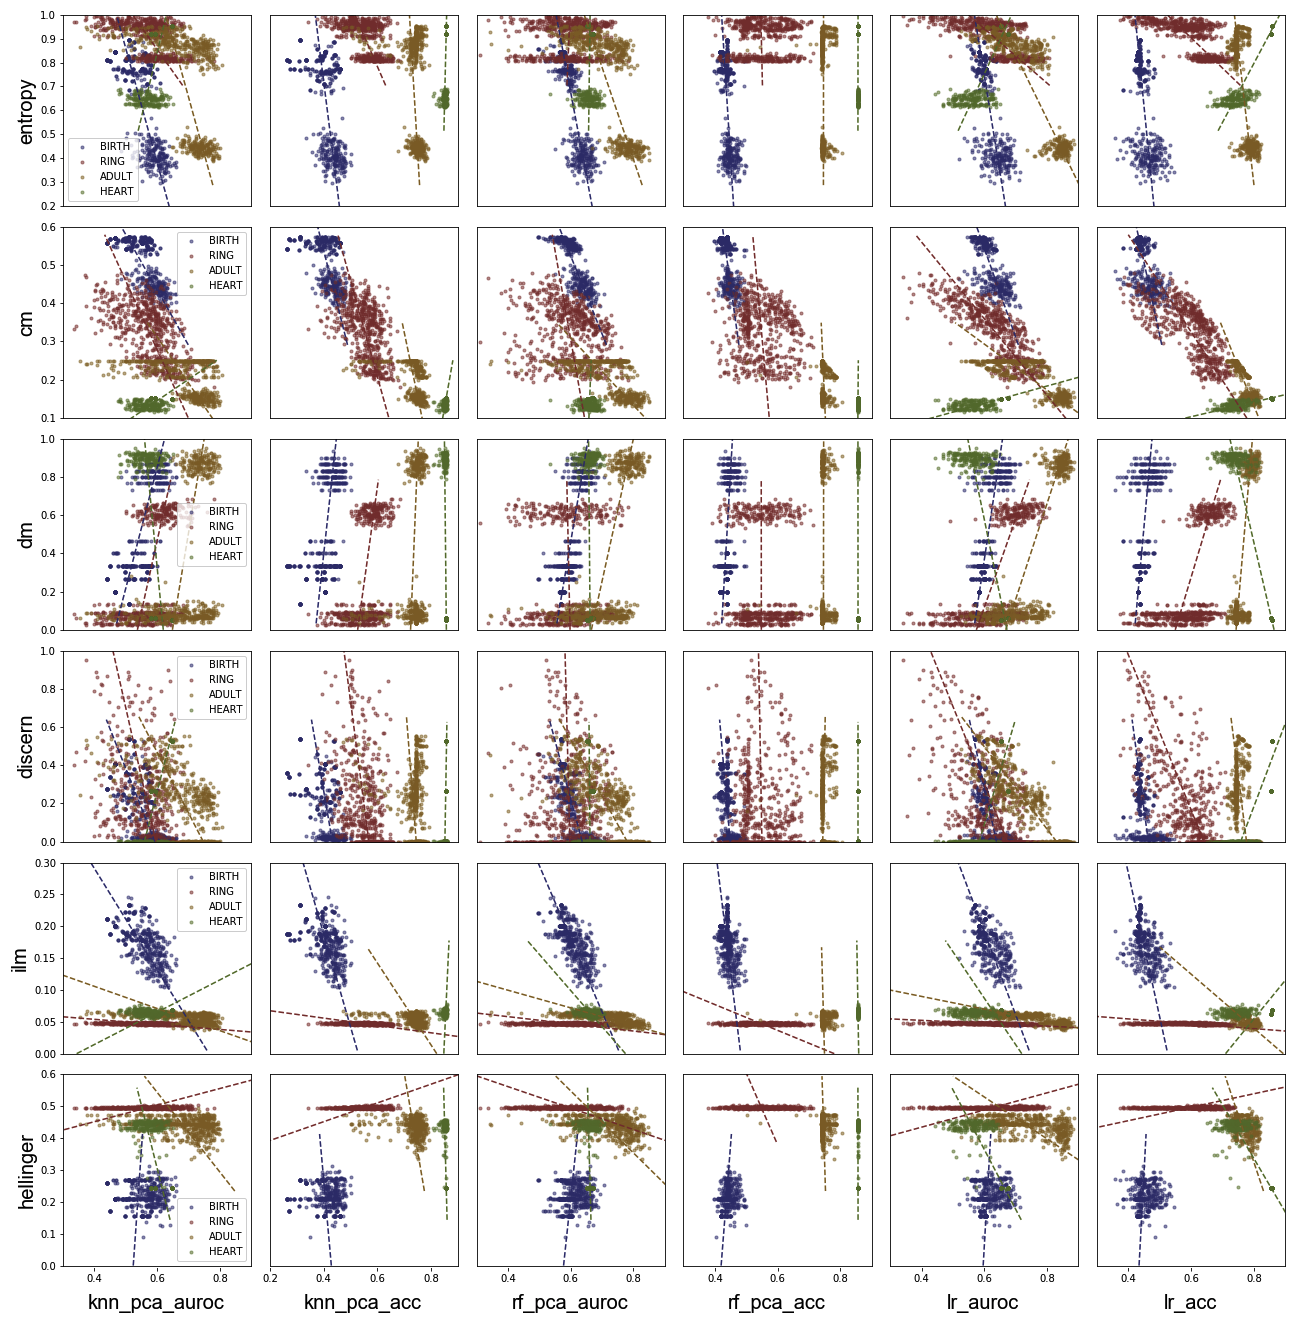
\includegraphics[width=1.2\textwidth]{project/fig/metrics-vs-accs_1.png}
    \caption{(Part 1) Scatterplots of the metrics against the classifiers for all datasets, separated by color. The dotted line is a line of best fit on a dataset obtained on all algorithms combined. We find separate clusters of points for every dataset caused by the difference in results for the different algorithms. Some metrics have consistent trends-- like the classification or diameter metrics -- across datasets, others, like the information loss metric, do not. We also look at the trends across classifiers used, and across the algorithms.}
    \label{fig:metrics_scatter1}
\end{figure}
\begin{figure}
    \centerfloat
    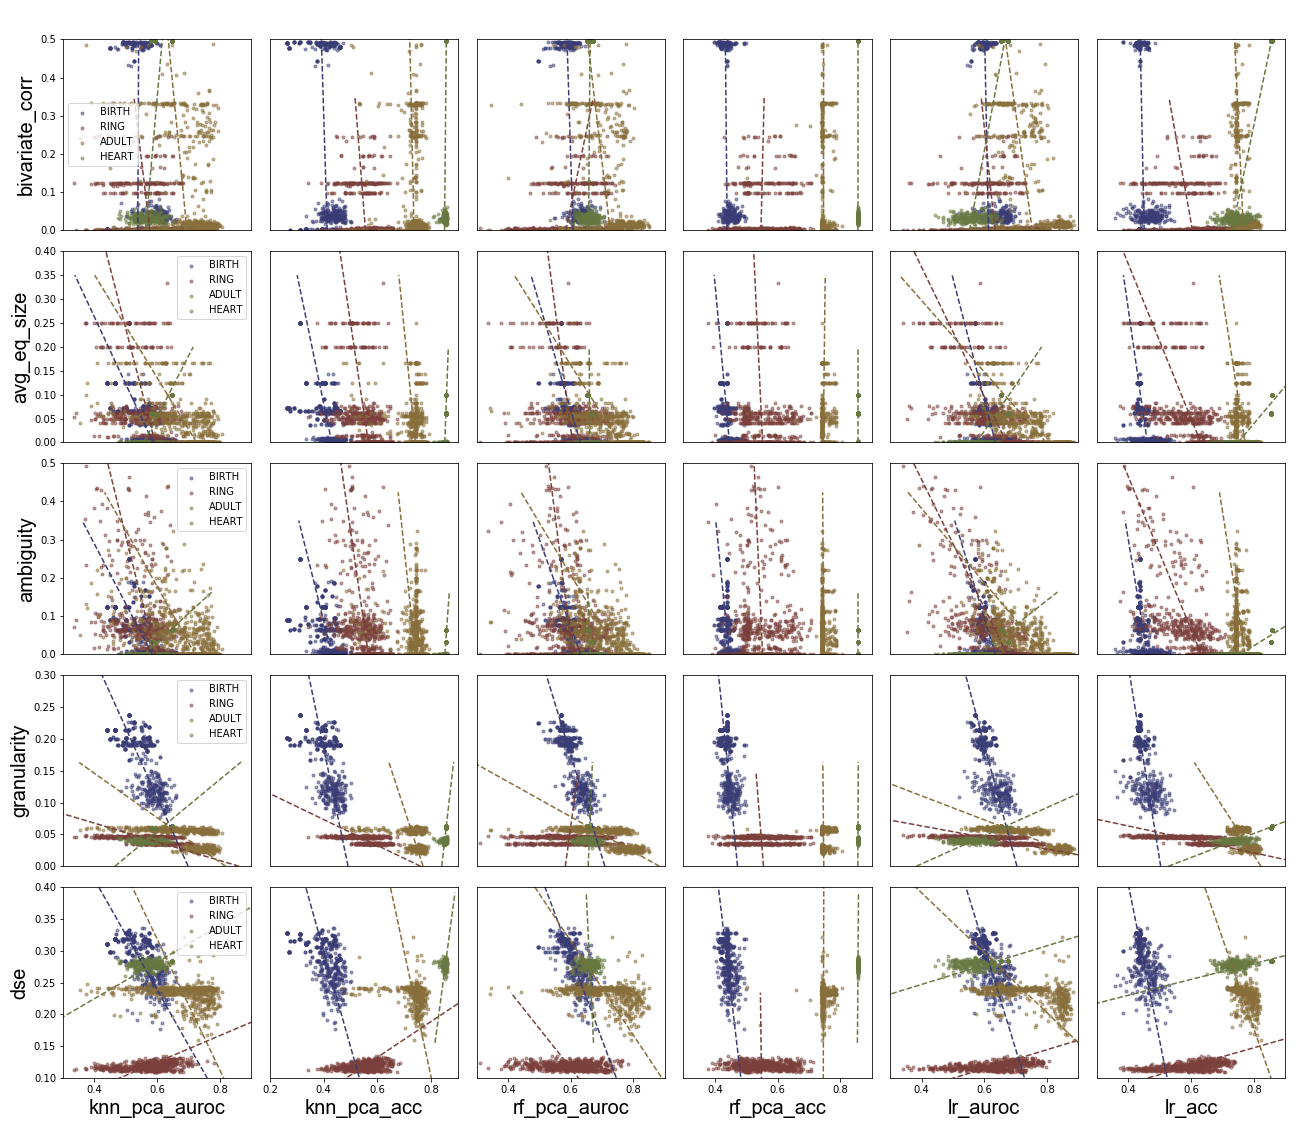
\includegraphics[width=1.2\textwidth]{project/fig/metrics-vs-accs_2.png}
    \caption{(Part 2) Scatterplots of the metrics against the classifiers for all datasets, separated by color. The dotted line is a line of best fit on a dataset obtained on all algorithms combined.}
    \label{fig:metrics_scatter2}
\end{figure}

\subsubsection{Disjoint Metric Clusters}
We first address the disjoint clusters found for every dataset: these are accounted for by the difference in algorithms. Mondrian outperforms the Datafly algorithms in terms of information preservation and this is reflected in the metrics. We can see the difference per algorithm more clearly in Figures \ref{fig:metric_hist1}, and \ref{fig:metric_hist2},  representing the distribution of metric results per algorithm used. 

In the metric distribution histograms mentioned above, we tend to see both Datafly algorithms heavily overlapping on their 200 respective datasets. While this is expected in metrics like \textbf{Entropy} that just quantify information loss, we do not spot major differences for metrics that actually look at the properties of the anonymous dataset-- the \textbf{Classification Metric}, for example. We would expect the equivalence classes in Datafly-Shuffled to have more diverse classification labels as we do not limit ourselves to grouping neighbouring, and thus similar, records. Nevertheless, we see that both Datafly algorithms are nearly overlapping, and so consistently across the datasets. This is unexpected as we designed the Datafly-Shuffled algorithm to intentionally lower its output's utility and it does not seem like it did.


\begin{figure}
    \centerfloat
    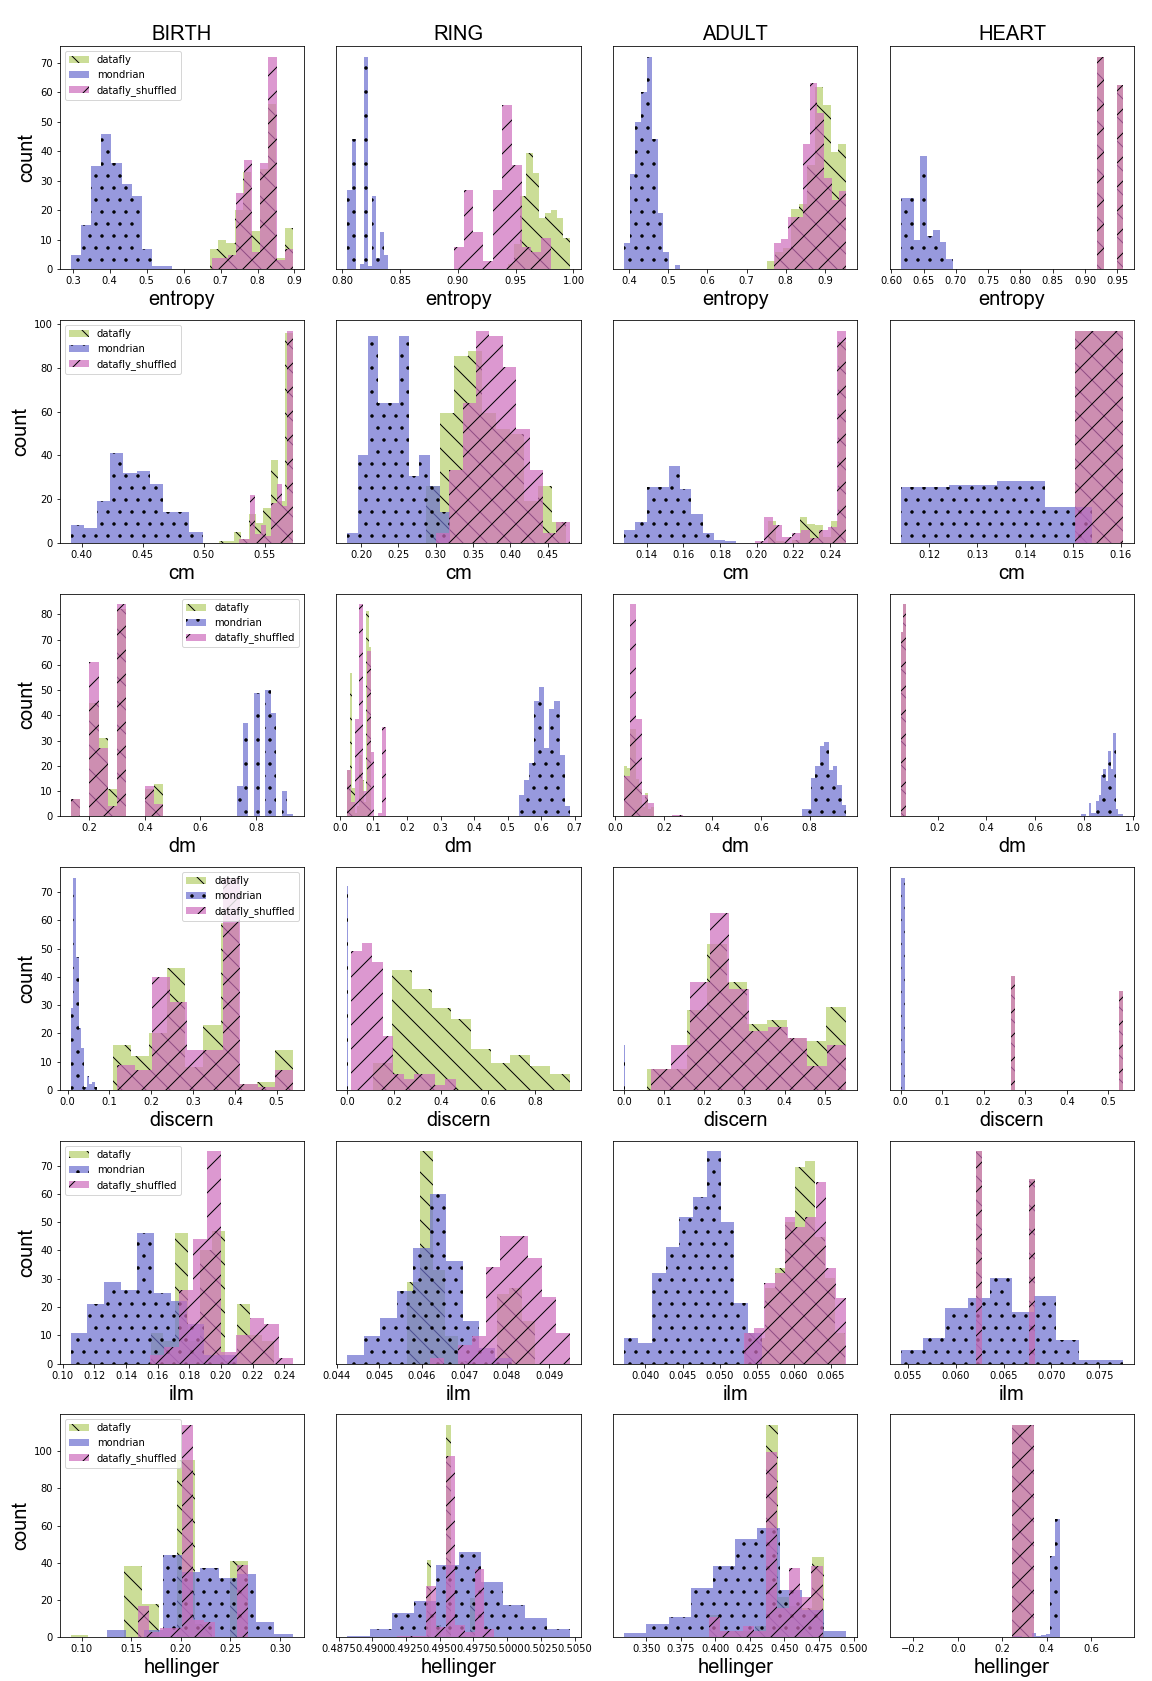
\includegraphics[width=\textwidth]{project/fig/metrics_hist_1.png}
    \caption{(Part 1) Histograms of the metrics over the four different datasets. The results show consistent overlap for the two Datafly algorithms while the Mondrian results stand apart.}
    \label{fig:metric_hist1}
\end{figure}
\begin{figure}
    \centerfloat
    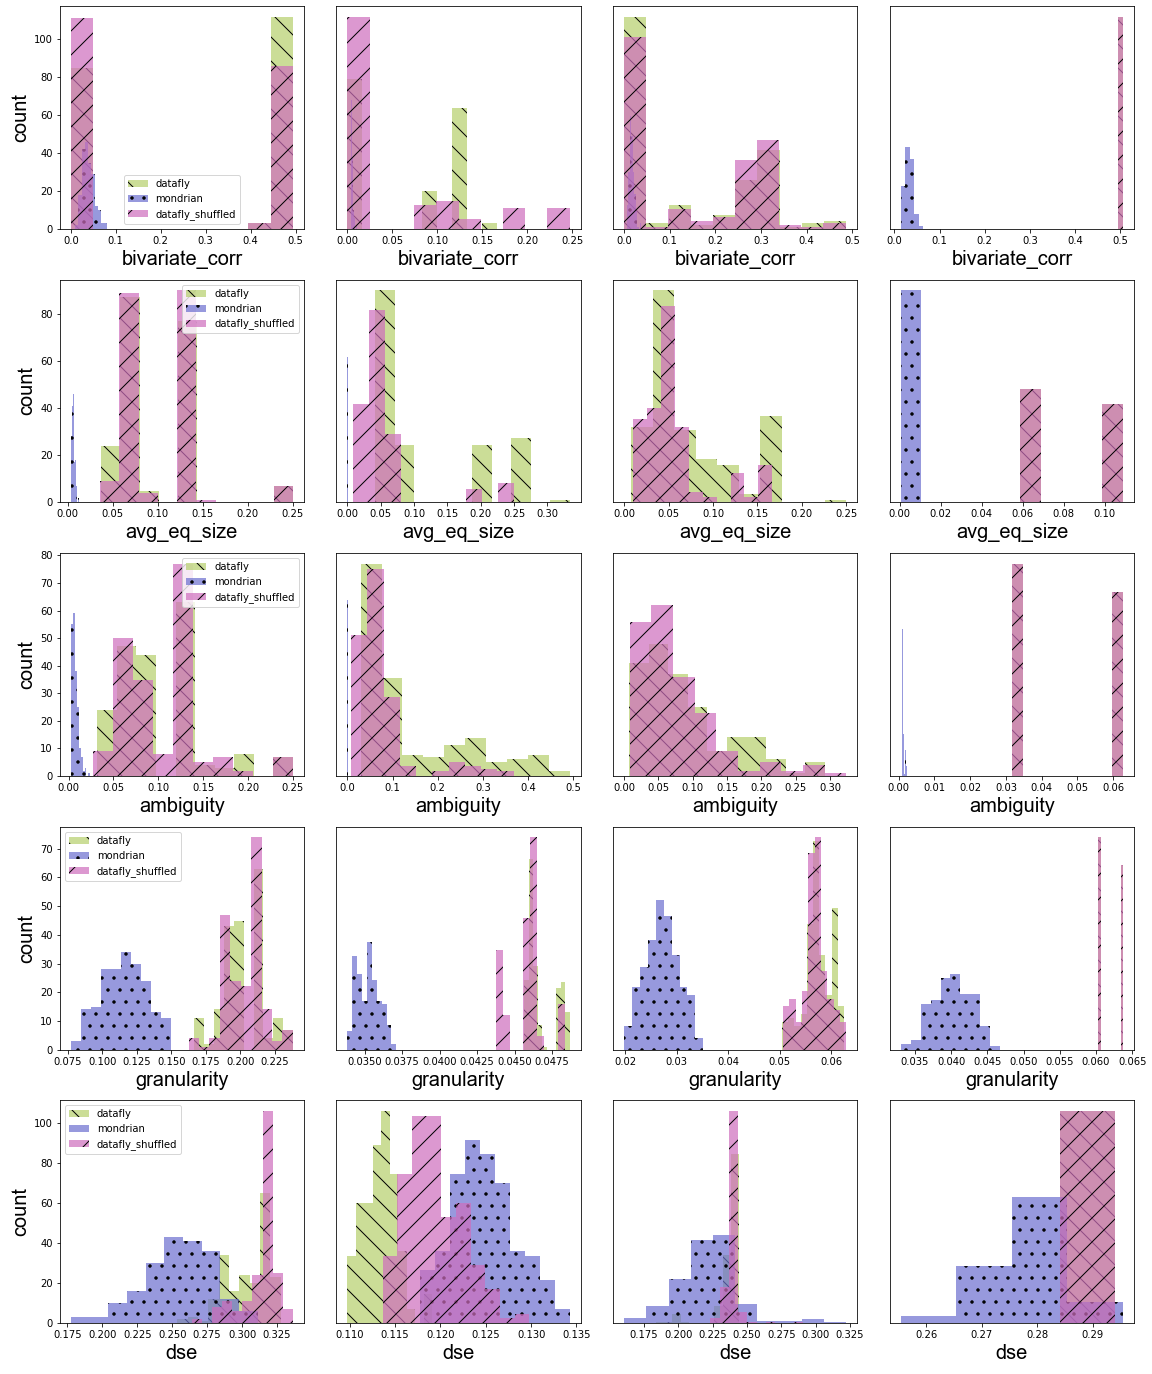
\includegraphics[width=\textwidth]{project/fig/metrics_hist_2.png}
    \caption{(Part 2) Histograms of the metrics over the four different datasets. The results show consistent overlap for the two Datafly algorithms while the Mondrian results stand apart.}
    \label{fig:metric_hist2}
\end{figure}

In Figure \ref{fig:hist_accs_perd}, we plot the distribution of the utility measures recorded on the different datasets and with the different algorithms. We observe that here, too, the Datafly-Shuffled datasets have very similar results to normal Dataflys datasets, allowing classifiers to perform equally well. The implication is that the classification metric did not differentiate between datasets of the two different algorithms because the two were inherently similar, and not because it is a bad metric.

The lack of difference in the shuffled and normal datafly datasets was surprising at first. Nevertheless, looking back at the datasets used, we found that this is due to the nature of the Datafly algorithm: it will generalize the attribute with the largest domain every time. Heuristically, this makes sense. However, it means binary attributes, like gender, are left untouched to the very end, due to their small ground domain size. All the while, the rest of the quasi-identifiers take heavy information losses. These binary attributes end up being the only non-suppressed values. On top of that, whether the binary attributes are switched or not is something any good classifier can work around. In short, the Datafly and Datafly-Shuffled datasets will tend to similar results because of how Datafly picks columns to generalize, and the fact it destroys most of the information that would create a difference between the modified algorithm and the original, even for small $k$ values, like $k=2$.

\begin{figure}
    \centerfloat
    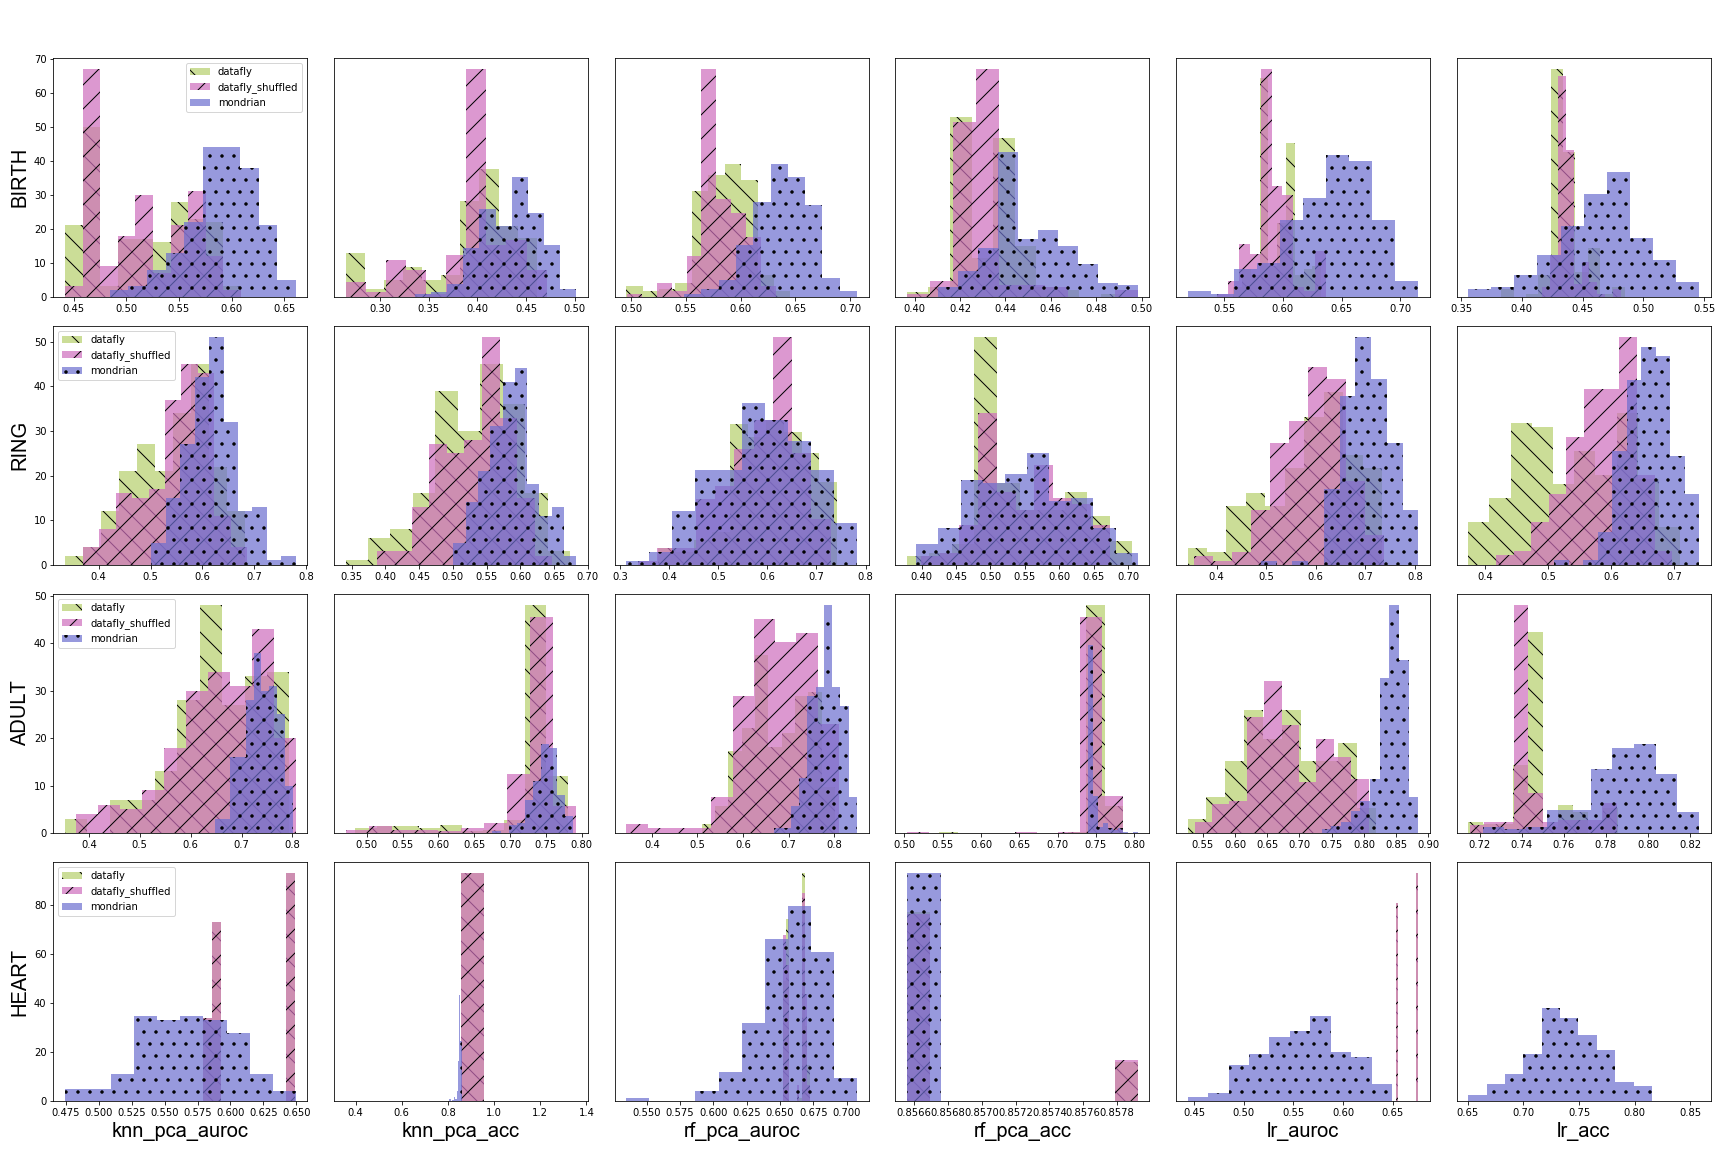
\includegraphics[width=1.2\textwidth]{project/fig/pat_full_accs.png}
    \caption{A set of histograms representing the distribution of measured utilities on different datasets (split by algorithm used). We see significant overlap on the two Datafly algorithms, and a tendancy for Mondrian datasets to score slightly higher than the others.}
    \label{fig:hist_accs_perd}
\end{figure}

\subsubsection{Trends for a Metric Across the Datasets}
\label{subsec:trends_datasets}
The metrics have varying success in getting consistent results across datasets. This can once again be seen in Figures \ref{fig:metrics_scatter1} and \ref{fig:metrics_scatter2}-- the scatterplots of the metrics for the different utility measures. 

Depending on the metric, when comparing the lines of best fits for the datasets in the same graphs, we get some mixed results. The \textbf{classification metric} manages to perform well: for all utility measures, all but the heart trend lines agree. Similarly so for the \textbf{diameter}, \textbf{average equivalence class size}, and a few other metrics. Nevertheless, the lines of best fit are not very pronounced (nearly vertical), implying little use for the metric: if, regardless of the metric score, we obtain the same utility, then the metric has zero predictive power. Other metrics do not do as well in terms of the consistency of their trends; the \textbf{hellingers}, \textbf{ilm}, and \textbf{squared distance error} metrics regularly have lines of best fit perpendicular to each other within the same graphs. This implies that even if a metric had predictive power on a dataset, it would be non-transferable to another, significantly reducing its real life applicability.

Furthermore, these trends are dataset wide and do not take into account the different algorithms. For example, looking at the \textbf{entropy} scatterplots (Fig. \ref{fig:metrics_scatter1}), we see the lines of best fit are influenced by having to connect the two disjoint clusters of different algorithms. If, instead, we fit a line per algorithm per dataset, we get Figures \ref{fig:sep_trends_gran} and \ref{fig:sep_trends_hell}, for the metrics of \textbf{granularity} and \textbf{hellinger}, respectively. For the sake of brevity, we do not include these figures for every metric, instead picking two good examples to illustrate this issue with the metrics. The full set of figures can be found in Appendix \ref{app:sep_trends_per_algo}. Notice that for the granularity metric (Fig. \ref{fig:sep_trends_gran}), lines of the same color (i.e., same dataset but different algorithms) are consistent; they have similar trajectories. 

However, when looking at the same plots for the \textbf{hellinger} metric (Fig. \ref{fig:sep_trends_hell}), we find a lot less consistency per dataset. For example, in the random forest accuracy plot (bottom, left), two out of the four datasets have nearly perpendicular trends on different algorithms. This occurs for most utility measures across this metric, particularly on the ring datasets (red).

\begin{figure}
    \centering
    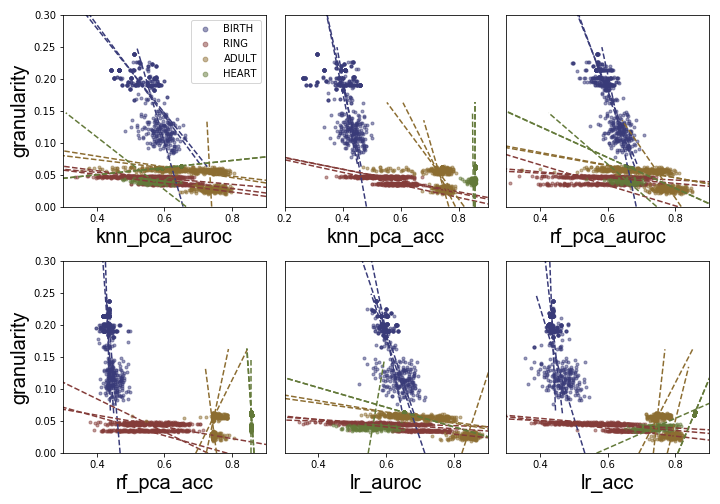
\includegraphics[width=0.8\textwidth]{project/fig/scatter_sep_trends/granularity_scatter.png}
    \caption{Scatterplots of the utility measures for the different classifiers against the granularity metric, separated by datasets. For every dataset, we draw a line of best fit per algorithm in order to show that lines for the different algorithms are consistent on the same datasets.}
    \label{fig:sep_trends_gran}
\end{figure}

\begin{figure}
    \centering
    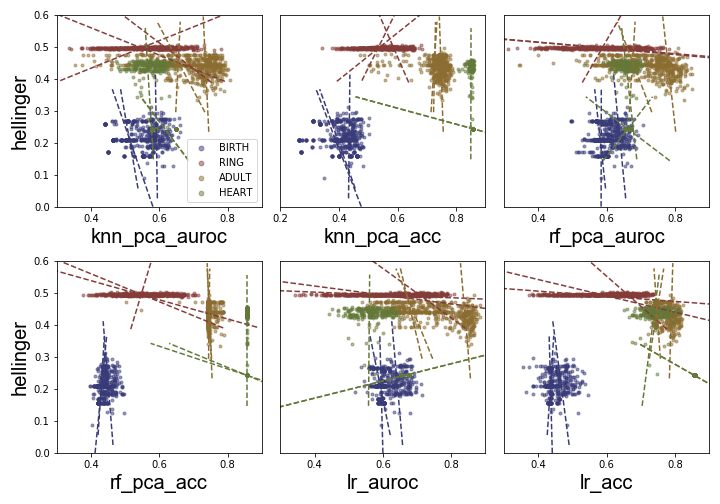
\includegraphics[width=0.8\textwidth]{project/fig/scatter_sep_trends/hellinger_scatter.png}
    \caption{Scatterplots of the utility measures for the different classifiers against the hellinger metric, separated by datasets. For every dataset, we draw a line of best fit per algorithm in order to show that lines for the different algorithms are \textbf{not} consistent on the same datasets.}
    \label{fig:sep_trends_hell}
\end{figure}

We mention this to highlight an issue with the metrics: their specificity-- we see that the trends are specific to the dataset, and furthermore, not all metrics are consistent based on the algorithm used. So, even starting from the hypothesis that metrics have some ability to predict dataset utility (which has not been convincing this far), before we could use metrics on a dataset, we would need to figure out what the trends are on that specific dataset. That means running experiments to figure it out, invalidating the whole point of metrics being an effortless way to predict utility.

\subsubsection{Trends for a Metric Across Classifiers}
Another dimension we can look at is whether the metric trends are consistent across the different classifiers and utility measures used. If this were the case, we could then argue that, at least, they have applicability irrespective of the classification task. We look at Figures \ref{fig:metrics_scatter1} and \ref{fig:metrics_scatter2} to compare the trends for the same datasets on different classification scores. For a metric to be useful, we need the trends for each dataset to be consistent across the row.

We find that the clearer the separation between the Datafly datasets and the Mondrian ones, the more consistent the lines of best fit are across the classifiers. For example, the \textbf{entropy} plots (Fig. \ref{fig:metrics_scatter1}, \ref{fig:metric_hist1}) show clear divisions between the metric results for Mondrian and Datafly results. This, in turn, forces the line of best fit to accommodate both sets of results and the larger the distance, the less variability we have in the slope of the best fit line. However, for metrics that have more overlap in the results for different algorithms-- like \textbf{Hellinger} (Fig. \ref{fig:metric_hist1}, \ref{fig:metrics_scatter1}), or \textbf{squared distance error} (Fig. \ref{fig:metric_hist2}, \ref{fig:metrics_scatter2}) metrics-- we find more variance in the lines of best fit. 

To remediate this, we create lines of best fit for the different algorithms. We refer, once again, to Figures \ref{fig:sep_trends_gran} and \ref{fig:sep_trends_hell}. These show that even though we have conditioned on the algorithm, we still have no consistency through the classification tasks. Looking at the \textbf{granularity} scatterplots (Fig. \ref{fig:sep_trends_gran}): the ring lines of best (red) fit stay consistent but because the metrics barely vary. We get some regularity for the birth datasets (blue), but very little for the adult dataset (yellow), alternating between positive and negative trends. We find equally erratic results on the \textbf{hellinger} metric scatters (Fig. \ref{fig:sep_trends_hell}), in which even the flat ring results (red) create lines of best fit seemingly randomly.


\subsubsection{No Linear Correlations}
We've mainly focused on the consistency of the lines of best fit throughout datasets/classifiers to test the applicability of metrics. Nevertheless, on top of consistency, we need the lines of best fit to contain some information. We find that a lot of trends that are very close to vertical, implying no linear correlation between the utility measures and metrics. For example, looking at metrics such as \textbf{bivariate correlation}, \textbf{diameter}, or \textbf{discernibility} in Figures \ref{fig:metrics_scatter1} and \ref{fig:metrics_scatter2} we find near vertical lines of best fit. In those cases, regardless of the metric score, the datasets have the same utility; it tells us nothing. Similarly, we find nearly horizontal lines for the ring dataset on information loss metrics: no matter the utility of a dataset, the metric spits out the same output, once again revealing nothing.


%\subsubsection{Summary of Scatterplots and Histograms}
%Through this section, we've seen that for a metric to be useful, it needs to be consistent no matter the dataset, the algorithm used, or the classification task. If it does not have these things, then it does not convey an interesting measure. On top of the consistency, it should also have some measure of correlation with the measured utilities, otherwise it has no value as a predictor.

%We find a few metrics that are relatively consistent through both the datasets, and the classifiers used: the classification, diameter, and average equivalence class size metrics. Nevertheless, we see the usefulness of the diameter metric drop because the trends are nearly vertical. The average equivalence class size has more pronounced trends, and so does the classification metric, although a lot more noisy.

%For most metrics, we double down on stating that they lack applicability due to their specificity. Based on what we've noted, if we wanted to use a metric to predict the utility of a dataset, we would need to do a lot of work to figure out the exact trend for the specific dataset being used. We would also need to ensure that the metric in question is consistent irrespective of the classifier used. To top it off, this is all based on the assumption that the metric has any predictive value, which isn't a given considering the metrics we've analyzed rarely fulfilled the criteria to be useful.

\subsection{Linear Regression: Metric Importance}
Using a different approach to assess the metrics, we attempt to find the most ``useful'' metric. We do this by fitting Linear Regressions on our standardized metrics, with the 6 model accuracies and AUROCs as the target variables. We consider the coefficients attributed to all the metrics. A larger coefficient implies a more significant impact on the regression, and, thus, more predictive power. Conditioning on the $k$-anonymization algorithm used and the dataset, we fit 72 linear regressions (4 datasets $\times$ 3 algorithms $\times$ 6 utility measures). 

For every metric, we measure the average effect size, and plot that in Figure \ref{fig:lin_reg}, along with the confidence intervals for these values. We find that the Average Class Size, Granularity, and Discernibility Metrics have the largest effect sizes. The Information Loss Metric is large too, but has an error margin that goes below most of the other metrics and their respective confidence intervals. The Hellinger, Bivariate Correlation, and Squared Distance Error are never the ones to have most added value.

Two metrics use the equivalence class sizes as a measure of utility: the Average Class Size Metric and the Discernibility Metric. The fact they both have large effect sizes indicate that equivalence classes are a good and easy way to assess a dataset's utility. Additionally, Average Class Size is amongst the metrics we recognized as potentially viable in the Single Metrics section, \ref{sec:single_metrics}.

Considering the way to measure utility was using classification tasks, it is surprising that the Classification Metric does not have larger effect sizes. It also had promising results in \ref{sec:single_metrics}. As a theoretical maximum measure, it might be that our classification tasks lacked the depth needed to achieve the optimal results, thus reducing the usefulness of the theory-based metric. 

The Hellinger, Bivariate Correlation, and Squared Distance Error Metrics bring up the rear in terms of largest average effect sizes. Hellinger and Bivariate, both presented by El Emam, et al., are ways to measure how the distributions of attributes change. This result might indicate that, in our usecase (i.e., a classification task), keeping attribute distributions constant is not a primary concern. Instead, based on the performance of the average equivalence class size, and discernibility metrics, we should shift our focus to how the records are grouped and generalized.

 
\begin{figure}[h]
    \centerfloat
    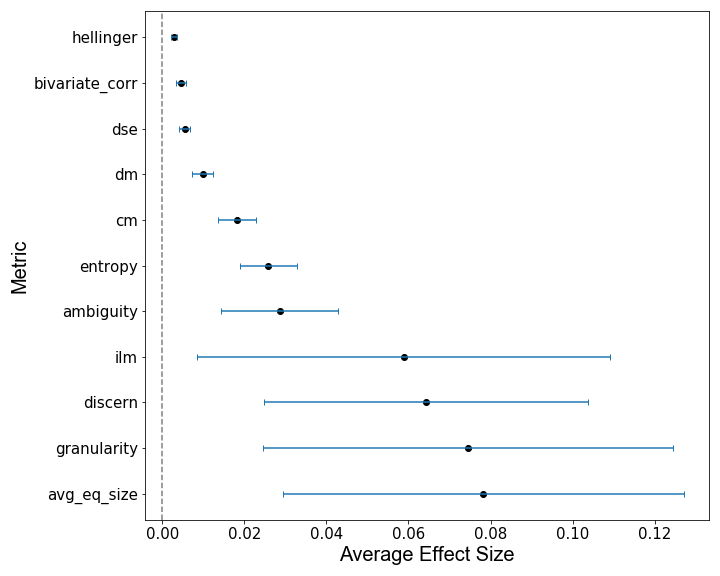
\includegraphics[width=0.8\textwidth]{project/fig/linreg_conf_interval.png}
    \caption{Fitting a linear regression on every utility measure, conditioned for dataset and algorithm, we measure the average effect size for the different metrics, along with the 0.95 confidence intervals. We find granularity, average equivalence class size, and discernibility to have higher effect sizes than the rest. However, their confidence intervals are equally large. Three metrics that measure distance, hellinger, bivariate correlation, and squared distance error, trail behind. All the confidence intervals are very large, but none pass over the $x=0$ line.}
    \label{fig:lin_reg}
\end{figure}


\subsection{1v1 Metric Prediction}
\label{sec:1v1_single}
As our analysis has been mostly qualitative in looking at the trends, we propose a more practical and quantitative way to test for a metric's use in predicting utility. The situation an analyst will often find themselves in is the following: given two $k$-anonymous datasets, which of the two should they use to maximize the utility? This will often happen when analysts use anonymization software like ARX \cite{arx}, for example. The platform allows you to easily modulate a few hyperparameters, and the actual anonymization is taken care of. The software outputs your anonymous dataset, and a list of metrics. 

In this case, the question becomes how much we should trust a metric, not based on a trend, but on a binary decision: we want to see how often, using a single metric, we can predict which dataset, out of two, has the most utility based on which has the best metric score. We then compare this to a baseline of a random choice, picking the best dataset 50\% of the time.

For every dataset and metric, we select $1000$ pairs of anonymous datasets in each algorithm used, and for every target utility measure. For every selected pair, we check if the dataset with the best metric score is also the one with the best utility measure. We then aggregate over the algorithm, and utility measures, to give a single rate per metric. 

%We condition on the algorithm because we notice that the metric results are always much better for the Mondrian datasets. Additionally, the Mondrian datasets generally outperform the Datafly sets as classification task training sets. Thus, if we compared a Mondrian to a Datafly, most of the time, it will have a better metric and a better utility. This is problematic as the metric comparison essentially turns into recognizing a Mondrian dataset from a Datafly one, a simpler task than predicting its utility. Instead, we look to compare identical algorithms only, averaging over the results.

\begin{table}
    \resizebox{\textwidth}{!}{%
    \begin{tabular}{|l|l|l|l|l|l|l|l|l|l|l|l|}
    \hline
    \rowcolor{gray!50}
    dataset & entropy & cm    & dm    & discern & ilm   & hellinger & bivariate\_corr & avg\_eq\_size & ambiguity & granularity & dse   \\ \hline
    \cellcolor{gray!50} birth   & 0.572   & 0.604 & 0.716 & 0.561   & 0.579 & 0.622     & 0.613           & 0.559         & 0.573     & 0.572       & 0.556 \\
    \cellcolor{gray!50} ring    & 0.593   & 0.644 & 0.591 & 0.587   & 0.604 & 0.621     & 0.573           & 0.562         & 0.599     & 0.605       & 0.554 \\
    \cellcolor{gray!50} adult   & 0.676   & 0.572 & 0.592 & 0.661   & 0.589 & 0.607     & 0.579           & 0.621         & 0.609     & 0.604       & 0.552 \\
    \cellcolor{gray!50} heart   & 0.752   & 0.774 & 0.768 & 0.747   & 0.748 & 0.872     & 0.728           & 0.748         & 0.748     & 0.75        & 0.742 \\ \hline
    \end{tabular}
    }
    \caption{A table displaying the rate of correctness when, comparing two $k$-anonymous datasets on a single metric, the anonymous dataset with the best metric score is also the one with the most utility. We see every metric predict at its best on the heart dataset, sometimes by large margins. Other than that, their predictive capacity is limited.}
    \label{tab:1v1_single_metrics}
\end{table}

We display the results in Table \ref{tab:1v1_single_metrics}. On the first three datasets (birth,ring,adult), the results are relatively similar-- scoring between 55.9\% and 71.6\%, and differing by a few percents inside the datasets. However, every metric predicts more accurately on the heart dataset than the others, correctly pointing to the dataset with the most utility around $75\%$ of the time. We believe this it might be due to the heavily unbalanced nature of the dataset. However, we merely offer it as a hypothesis as we have no proof to back it up.

Comparing the results to a random choice, we find the odds using metrics are better, but only marginally so.

This practical test provides a good place to wrap up the analysis of metrics individually. We have observed that metrics can separate a $k$-anonymous dataset anonymized using Mondrian from one anonymized with either of the Datafly algorithm. However, once the algorithm is fixed, no metric can consistently and successfully pick a dataset that has managed to retain more utility than other-- we only get a marginal increase in the probability of picking the correct one. As such, these metrics are not ideal tools to assess utility after a $k$-anonymization. Until an alternative is proposed, metrics could be used, but should always be taken with a grain of salt.


\section{Meta-Metrics}
As described in section \ref{sec:metametrics}, we aim to show that even tapping their full potential, metrics are only so predictive. We train a Meta-Metric-- an Auto-Sklearn ensemble model-- per combination of dataset, algorithm, and utility measure. We then use a test set of metrics to measure the accuracy of our Meta-Metric in predicting the utility of a dataset. We plot the Meta-Metrics' predicted utilities against the real measured utility as scatterplots on the different datasets and utility measures in Figure \ref{fig:meta_scatter}. Every color represents the Meta-Metric for a specific algorithm. The results show that most of the Meta-Metrics are good utility predictors because the trend lines are regularly close to the reference $y=x$ line. We generally find good trends but noisy results. 

%Normal Scatter
\begin{figure}
    \centerfloat
    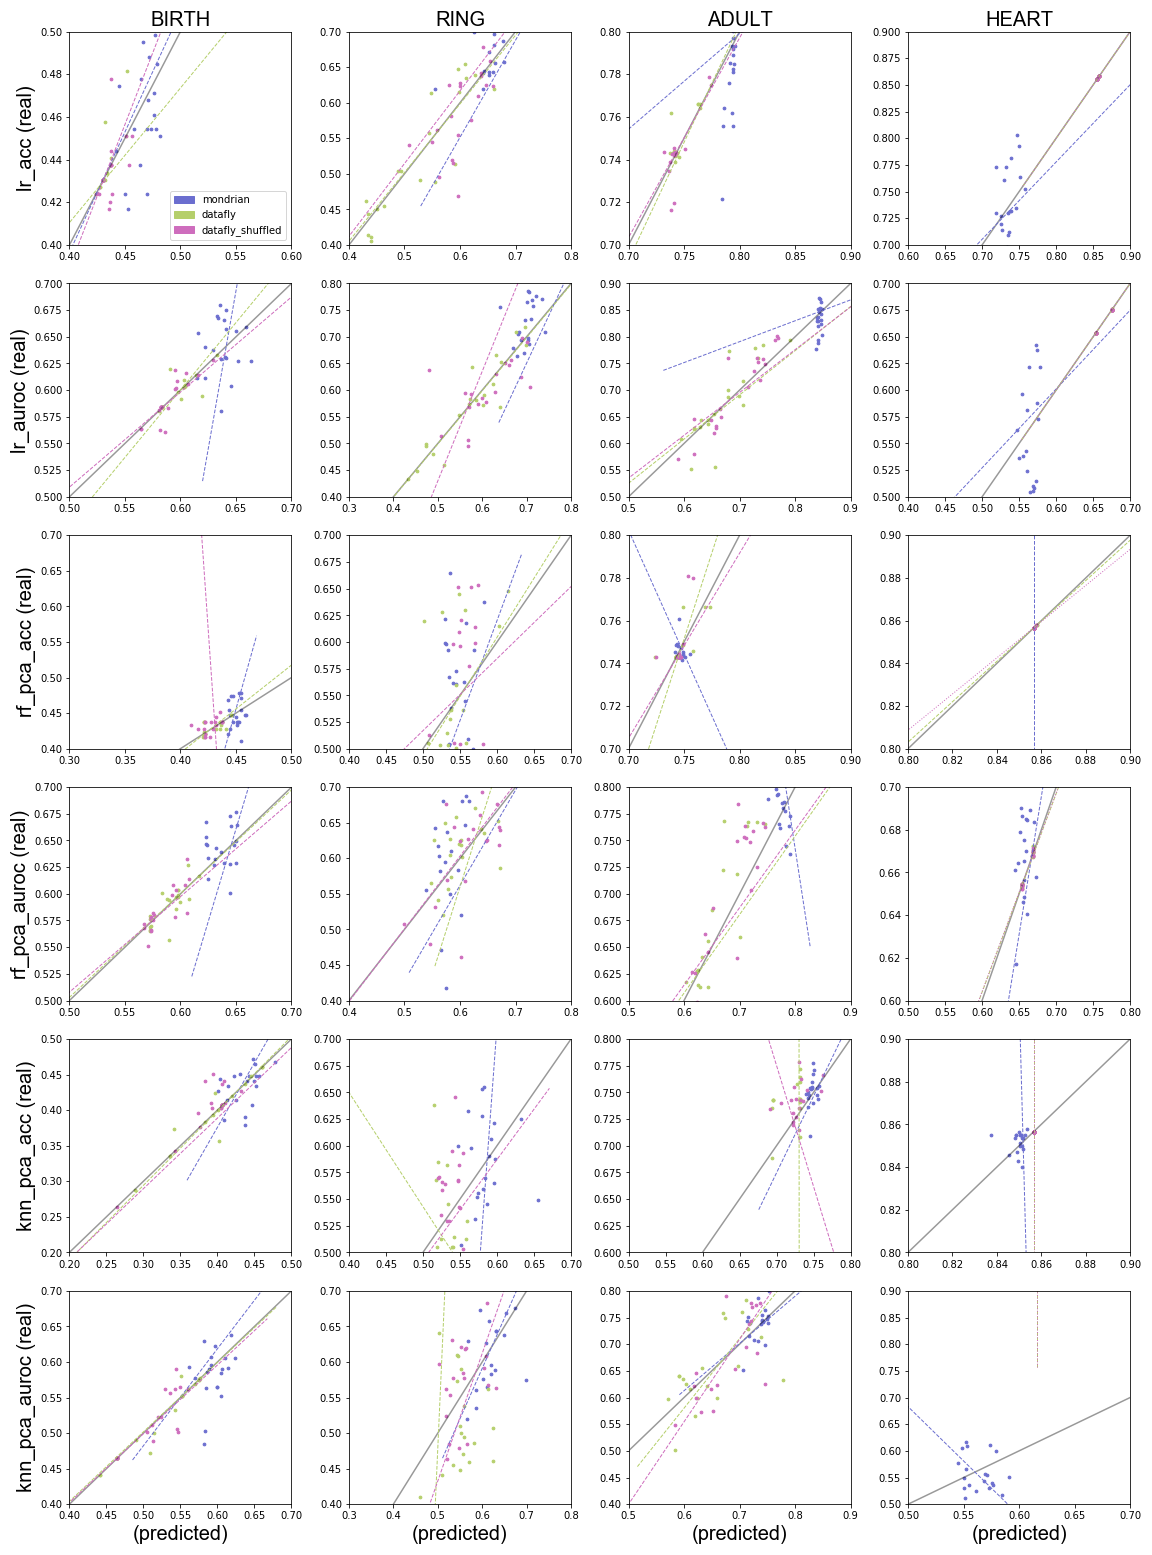
\includegraphics[width=\textwidth]{project/fig/megametrics-vs-accs_sep_trends.png}
    \caption{Scatterplots of the Meta-Metrics-- the trained Auto-Sklearn ensemble models-- predicting utility for the different algorithms on the different datasets. The different colors represent the different algorithms. The thin black line is the reference $y=x$ line, and the colored dashed lines are the trend lines for the scatters. The results show most Meta-Metrics predicting true utility reasonably accurately, with a few exceptions, notably on the heart datasets.}
    \label{fig:meta_scatter}
\end{figure}


\subsection{1v1 Meta-Metric Prediction}
As a more quantitative analysis of the Meta-Metrics, we replicate the method described in section \ref{sec:1v1_single}: when given two random datasets, what are the chances that the dataset with the highest Meta-Metric score is the one that is most ``useful''? We take the test set saved for every combination of algorithm, dataset, and utility measure, and compare the predicted utility to the measured utility. We then take the average of the results for the utility measures to aggregate by algorithm in Table \ref{tab:1v1_meta}. 

Depending on the dataset, we get different performances. We do not see much improvement on the ring dataset-- its highest single metric scored picked the most useful dataset 64.4\% percent of the time, and the combined metrics only increased that by 0.5\%. Adult has a lower average score than the single metric entropy for that dataset did. However, the average sees some improvement compared to its single metric results, averaging 66.7\% using the Meta-Metrics compared to a previous average of 60.5\%. Birth sees a larger increase, picking correct datasets about 76\% of times. The heart dataset once again scores better on all the algorithms than the others.

Putting things back into perspective, the Meta-Metrics generate an increase of the percent of times we pick the dataset with most measured utility, but still with mixed success. This is probably due to the noise we obtained, seen in the scatterplots. The overall trend is good, but when picking out a dataset from a handful of them, it becomes much harder. Considering that this is a best case scenario, the results paint a bleak picture for metrics.

\begin{table}[h]
\begin{tabular}{|l|c|}
\hline
\rowcolor{gray!50}
\cellcolor{gray!50} Dataset & Avg. Correctness  \\
\hline
\cellcolor{gray!50} birth   & 0.763 \\
\cellcolor{gray!50} ring    & 0.649 \\
\cellcolor{gray!50} adult   & 0.667 \\
\cellcolor{gray!50} heart   & 0.883 \\
\hline
\end{tabular}
\centering
\caption{A table displaying the rate of correctness of the 1v1 experiments on the Meta-Metrics. Here, we aggregate on the utility measures and algorithms to display results per dataset. Results show our Meta-Metrics predict more accurately than the individual metrics, but not by much.}
\label{tab:1v1_meta}
\end{table}




\subsection{Meta-Metric ``Transferability''}
Not only do we show that even the Meta-Metrics struggle to consistenly make good decisions, but we show that they become even more inconsistent as soon as we try to transfer their predictive powers to other tasks. To show the lack of Meta-Metric reusability, we tailor the 1v1 comparison method previously used. 

The intuition is as follows: if we cannot use a Meta-Metric trained to predict utility for Mondrian datasets to predict the best of two datasets that were anonymized using a Datafly algorithm (keeping the dataset type and utility measure constant), then the Meta-Metric is specific to Mondrian, and equally so for the other algorithms. This implies that if we wanted to use Meta-Metrics as utility metrics, we would need one Meta-Metric per algorithm in existence. 

On top of that, we need to ensure that the Meta-Metrics are also transferable to other dataset. In other words, using the Meta-Metric trained for a particular type of dataset (e.g., birth, ring,...), out of two datasets from another type of dataset, can we still apply our Meta-Metric to pick the most useful? If we cannot, that once again implies we need a Meta-Metric per type of existing dataset, of which there are infinitely many.

Finally, the same problem applies to the utility measure-- there are infinitely many classification tasks. If a Meta-Metric trained for a specific utility measure cannot be used to help predict other utility measures then the Meta-Metrics cannot be useful.

For Meta-Metrics to be useful as predictors of utility, we would need to show that they are transferable across three dimensions: algorithm used, dataset type, and utility measure. Therefore, we do three experiments:

\begin{itemize}
    \item Given two $k$-anonymous datasets anonymized using a specific algorithm, can we predict the one with more utility using a Meta-Metric trained on another algorithm?
    
    \item Given two $k$-anonymous datasets, can we predict the one with more utility using a Meta-Metric trained on another dataset?
    
    \item Given two $k$-anonymous datasets, can we predict which will have a better measured utility using a Meta-Metric trained for another utility measure?
\end{itemize}

We keep every dimension not being tested constant. For example, testing if the Meta-Metric trained on the Datafly algorithm transfers to the Mondrian and Datafly-Shuffled algorithm, we only test the Meta-Metric of the combination (Datafly $\times$ birth $\times$ lr\_acc) on $k$-anonymous versions of birth datasets, and using the lr\_acc utility measure.

All three questions result in the same answer: the Meta-Metrics cannot be transfered; taken out of their context, they do not have any use. 


\subsubsection{Are the Meta-Metrics transferable to other algorithms?}
To test if the Meta-Metrics trained on a specific algorithm are transferable, for every Meta-Metric trained on that algorithm, we filter the test metrics to those that were for different algorithms, but the same dataset. We then use the Meta-Metric to predict their utility, and ,for every pair of datasets, check to see if the one with the best predicted utility is the one that is truly most useful. Aggregating on all the datasets and utility measures, we find the percentage of time the Meta-Metrics correctly predict the most useful of two datasets. The information is displayed in Table \ref{tab:1v1_cross_algo}. 

The results show a lack of transferability for Mondrian Meta-Metrics to the other algorithms' datasets; they correctly identify the better dataset 60\% of the time (or about 10\% better than random). The Datafly algorithms are more transferable between each other which makes sense as they obtained similar results throughout our experiments. Nevertheless, because of the similarity of the results seen throughout this project, we would have expected the portability of the Datafly Meta-Metrics to and from the Datafly-Shuffled Meta-Metrics to be better. We conclude Meta-Metrics are algorithm specific.

\begin{table}[h]
\center
\begin{tabular}{|c|l|l|l|}
\hline
\rowcolor{gray!50}
Meta-Metric used \textbackslash used on  & mondrian & datafly & datafly\_shuffled \\
\hline
\cellcolor{gray!50} mondrian          & -        & 0.606   & 0.607             \\
\cellcolor{gray!50} datafly           & 0.668    & -       & 0.765             \\
\cellcolor{gray!50} datafly\_shuffled & 0.631    & 0.823   & -      \\
\hline
\end{tabular}
\caption{A table to show how often, when using the Meta-Metric for one algorithm, we could predict the most useful of two datasets that have been anonymized using another algorithm. We find that Mondrian does not predict Datafly datasets very well, and Datafly algorithms do not perform well on Mondrians either.}
\label{tab:1v1_cross_algo}
\end{table}

\subsubsection{Are the Meta-Metrics transferable to other datasets?}
We conduct a similar experiment for the transferability of Meta-Metrics to other datasets as we did for the transferability to other algorithms: we test how well the Meta-Metric for a dataset can predict the most useful of two datasets, of a different type, but anonymized by the same algorithm and with the same utility measure. We display the percentages obtain for the different Meta-Metrics in Table \ref{tab:1v1_cross_sets}.

The results show that the Meta-Metrics on one dataset struggle to make sense of the metrics calculated on another type of dataset, never scoring above 78.1\%. We come to the conclusion that Meta-Metrics are dataset specific as well.
\begin{table}[h]
    \center
    \begin{tabular}{|c|l|l|l|l|}
\hline
\rowcolor{gray!50}
Meta-Metric dataset \textbackslash used on & birth & ring  & adult & heart \\
\hline
\cellcolor{gray!50} birth   & -     & 0.567 & 0.583 & 0.719 \\
\cellcolor{gray!50} ring    & 0.696 & -     & 0.641 & 0.781 \\
\cellcolor{gray!50} adult   & 0.585 & 0.627 & -     & 0.75  \\
\cellcolor{gray!50} heart   & 0.723 & 0.671 & 0.75  & - \\
\hline
\end{tabular}
    \caption{A table to show how often, when using the Meta-Metric for one dataset, we could predict the most useful of two $k$-anonymous datasets from another original set. We find that the Meta-Metrics do not transfer well across dataset, as no score is above a 78\%.}
    \label{tab:1v1_cross_sets}
\end{table}

\subsubsection{Are the Meta-Metrics transferable to other utility measures?}
Finally, we test to see if training Meta-Metrics for one utility measure is enough or if they are task specific. We follow the same procedure as above, this time keeping the datasets and algorithms constant, and obtain the results displayed in Table \ref{tab:1v1_cross_measures}. These are condemning results for the usefulness of Meta-Metrics (and by implication information loss metrics in general): We see that no Meta-Metric trained for a certain type of utility measure can be used to pick a more useful dataset out of two for another measure. The best performing cross measure Meta-Metric barely scored 22\% better than random.

\begin{table}[h]
\centerfloat
\resizebox{\textwidth}{!}{%
\begin{tabular}{|c|l|l|l|l|l|l|}
\hline
\rowcolor{gray!50}
Meta-Metric used \textbackslash used to predict & lr\_acc & lr\_auroc & rf\_pca\_acc & rf\_pca\_auroc & knn\_pca\_acc & knn\_pca\_auroc \\ \hline
\cellcolor{gray!50} lr\_acc & - & 0.554 & 0.721 & 0.507 & 0.673  & 0.63 \\
\cellcolor{gray!50} lr\_auroc  & 0.611  & - & 0.696 & 0.696 & 0.642  & 0.58 \\
\cellcolor{gray!50} rf\_pca\_acc & 0.632  & 0.646  & - & 0.627 & 0.652  & 0.558 \\
\cellcolor{gray!50} rf\_pca\_auroc & 0.576   & 0.727 & 0.685 & - & 0.622  & 0.607  \\
\cellcolor{gray!50} knn\_pca\_acc & 0.705  & 0.648   & 0.708 & 0.623 & - & 0.638 \\
\cellcolor{gray!50} knn\_pca\_auroc & 0.643 & 0.701 & 0.723 & 0.701 & 0.645  & - \\ 
\hline
\end{tabular}}
\caption{A table to show how often, when using the Meta-Metric trained for one utility measure, we could predict the most useful of two $k$-anonymous datasets according to another utility measure. We find that the Meta-Metrics do not transfer well across dataset, as no score is above a 73\%.}
\label{tab:1v1_cross_measures}
\end{table}

These results imply that Meta-Metrics are not very versatile tools. They can only be used in the exact context they were trained for.



\subsection{Implications for Individual Information Loss Metrics}
The Auto-Sklearn models learned how to combine the strengths of every individual metric in an optimal way, and while on a specific task-- a combination of algorithm, dataset, and utility measure-- the resulting trends were promising, we show that, when used to pick a dataset from a handful of choices, their predictive power takes a hit.

As a result of our experiments, we show that we cannot use the Meta-Metrics created here on random $k$-anonymized datasets or for any other combination of algorithm, dataset, and classification task than those presented here. As such, we come to the conclusion that if even the Meta-Metrics cannot be used out of their context, then no single metric will be usable either as no single metric at its best is better than all the metrics at their best.